
%%%%%%%%%%%%%%%%%%%%%
\section{Chute libre}
%%%%%%%%%%%%%%%%%%%%%
%
\subsection{Définition}

On lache une balle. On observe que celle-ci se met en mouvement, se dirige vers le bas, puis frappe le sol. Cette succession d'évènements constitue un phénomène : le phénomène de la chute libre.

\subsection{Paradigmes}

Il existe plusieurs paradigmes qui tente de donner une explication rationnelle à ce phénomène. Pour aristote, la balle constituée de matière terrestre souhaite rejoindre le lieu de la matière terrestre qui est le bas. Pour Newton, la force gravitationnelle entre la Terre et la balle provoque la mise en mouvement de la balle. Pour Lagrange et Hamilton, l'énergie potentielle de gravitation de la balle se convertie en énergie cinétique. 


L'énergie potentielle est relié à la position, l'énergie cinétique est relié au mouvement, à la vitesse.

%\begin{center}
%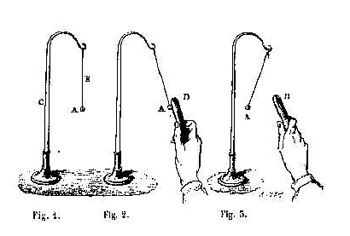
\includegraphics[scale=0.9]{./theorieDesChamps/MascartTraiteDElectriciteStatique1876}
%\end{center}

L'expérience du pendule électrostatique peut se modéliser par des {\it forces électrostatiques} s'exerçant entre les particules chargées. Ce modèle suppose une {\it action à distance}. La notion de champs permet de modéliser cette action entre les charges électriques : une charge électrique crée un champ dans tout l'espace. Le champ exercent une force sur les charges électriques.

% Dans un second temps, elle peut se modéliser par  en disant qu'une particule chargée crée un champ électrostatique en tout point de l'espace et qu'une particule chargée placé dans un champ électrostatique subit une force.

%\begin{minipage}[c]{.45\linewidth}
\begin{center}
Vision "Force de Gravitation"
\end{center}
La Terre exerce une force de gravitation $\overrightarrow{F}_{T/B}$ sur la balle $B$
\setlength{\unitlength}{1cm}
\begin{picture}
\shade[top color=blue, bottom color=lightgray] (0,0) arc (105:75:25) -- cycle;
%\put(0.5,1.0){\circle{0.3}}
\put(0.3,-0.3){$Terre$}

\put(5.5,1.0){\circle{0.5}}
\put(5.3,0.2){$B$}
\put(5.5,1.0){\vector(-1,0){1.36}}
\put(3.7,1.3){$\overrightarrow{F}_{T/B}$}
\end{picture}
%\end{minipage}
%\hfill
%\begin{minipage}[c]{.45\linewidth}
\begin{center}
Vision "Énergétique"
\end{center}
La balle possède une énergie potentielle de gravitation lié à son altitude, au cours de sa chute, elle acquiert une énergie cinétique lié à sa vitesse. Au cours de la chutte, l'énergie potentielle est convertie en énergie cinétique. L'énergie totale, reste constante.
\setlength{\unitlength}{1cm}
\begin{picture}(10,3)
\put(0.5,1.0){\circle{0.3}}
\put(0.3,0.3){$Q_1$}
\put(5.5,1.0){\vector(-1,0){1.36}}
\put(3.7,1.3){$\overrightarrow{E}$}
\end{picture}
Le champ électrique $\overrightarrow{E}$ exerce une force $\overrightarrow{F}_{\overrightarrow{E}/Q_2}$ sur la charge électrique $Q_2$
\setlength{\unitlength}{1cm}
\begin{picture}(10,3)
\put(5.5,1.0){\circle{0.5}}
\put(5.3,0.2){$Q_2$}
\put(5.5,1.0){\vector(-1,0){1.36}}
\put(3.7,1.3){$\overrightarrow{F}_{\overrightarrow{E}/Q_2}$}
\end{picture}
%\end{minipage}

%\subsection{Champ magnétique}

%%%%%%%%%%%%%%%%%%%%%%%%%%%%%%%%%%%%%%%%%%%%%%%%%%%%%%%%%%%%%%%%%%%%%%%%%%%%
